% Compile with: pdfLaTeX -> Biber -> pdfLaTeX -> pdfLaTeX
% This manuscript uses APA author-date citations in an IEEE two-column layout.
\documentclass[conference]{IEEEtran}

\usepackage[T1]{fontenc}
\usepackage[utf8]{inputenc}
\usepackage{lmodern}
\usepackage{microtype}
\usepackage{amsmath,amssymb}
\usepackage{booktabs}
\usepackage{tabularx}
\usepackage{multirow}
\usepackage{graphicx}
\usepackage{tikz}
\usetikzlibrary{arrows.meta,positioning,shapes.geometric,fit}
\usepackage{algorithm}
\usepackage{algpseudocode}
\usepackage{csquotes}
\usepackage[style=apa,backend=biber,sorting=nyt,maxcitenames=2]{biblatex}
\DeclareLanguageMapping{english}{english-apa}
\addbibresource{references.bib}
\setlength{\emergencystretch}{2em}

\title{STP-RAG: Semantic Transition Profile Guided Adaptive Chunking and Context Selection for Long-Document Retrieval-Augmented Generation}

\author{\IEEEauthorblockN{Author Name 1, Author Name 2, and Author Name 3}
\IEEEauthorblockA{Department of Computer Science and Engineering\\
Institution Name, City, Country\\
\{author1, author2, author3\}@example.edu}}

\begin{document}
\maketitle

\begin{abstract}
Retrieval-augmented generation (RAG) depends on chunk representations that expose relevant evidence without severing the context needed to interpret it. Fixed windows and single-threshold semantic chunking impose one segmentation policy on document regions that may be stable, abruptly changing, or locally volatile. This paper introduces the \emph{Semantic Transition Profile} (STP), a local representation of document dynamics that combines semantic velocity, semantic acceleration, semantic volatility, and structural cues. STP-RAG uses this shared profile to guide boundary selection, target chunk length, and the amount of preceding context considered for selective propagation. The retrieval stage is deliberately treated as a downstream evaluation environment rather than claimed as a new retrieval paradigm. We formulate the method, specify reproducible implementation choices, and define an empirical protocol that compares fixed, similarity-based, velocity-only, and progressively richer STP variants. The manuscript reports no fabricated results: all result cells are explicitly reserved for measurements from the implemented system. The central research question is whether modelling the \emph{pattern} of local semantic change produces more useful RAG representations than relying on a single adjacent-unit similarity value.
\end{abstract}

\begin{IEEEkeywords}
retrieval-augmented generation, semantic chunking, adaptive chunking, document embeddings, long-context retrieval
\end{IEEEkeywords}

\section{Introduction}
Retrieval-augmented generation combines a parametric generator with non-parametric evidence retrieved from an external corpus \parencite{lewis2020retrieval}. In long documents, the quality of this evidence is influenced substantially by the representation chosen before retrieval. Chunks that are too large can mix unrelated claims and lower retrieval precision; chunks that are too small can separate a statement from its definitions, conditions, or exceptions. This tension remains relevant even as embedding models and retrievers improve \parencite{karpukhin2020dense,gao2024retrieval}.

Many practical RAG systems divide text by a fixed token budget, recursive separators, headings, or adjacent-sentence similarity. These strategies are useful baselines, but they do not explicitly distinguish a stable topical region from a region entering an abrupt transition or a region with repeated local shifts. A single semantic distance can be high in both cases, even though the appropriate segmentation and context policy may differ.

This work studies a narrower and testable proposition: local semantic change can be represented as a reusable control signal. For ordered textual units, STP combines the rate of semantic displacement (velocity), the change in that rate (acceleration), the local variation of the rate (volatility), and document-structure features. It then uses the profile to control three document-preprocessing decisions: boundary probability, target chunk budget, and context horizon. Figure~\ref{fig:architecture} summarizes the intended pipeline.

The contribution is not a claim that embeddings, adaptive chunking, or multi-stage retrieval are individually new. Adaptive retrieval and content-aware chunking are active research areas \parencite{gao2024retrieval,edge2024local}. Instead, the paper contributes a concrete formalisation and an evaluation plan for using one transition profile across normally separate preprocessing choices. The paper makes four contributions:
\begin{enumerate}
    \item It defines STP using velocity, acceleration, volatility, and structural cues over a sequence of document-unit embeddings.
    \item It derives an adaptive boundary and granularity policy from the profile while enforcing minimum and maximum chunk budgets.
    \item It introduces a selective, STP-guided context-horizon policy intended to preserve useful dependencies without attaching a fixed amount of history to every chunk.
    \item It provides a reproducible experimental and ablation protocol. Results are left blank until obtained from real runs, avoiding unsupported empirical claims.
\end{enumerate}

\section{Related Work}
\subsection{Retrieval-Augmented Generation and Dense Retrieval}
RAG was introduced as a framework in which retrieved documents complement a sequence-to-sequence generator \parencite{lewis2020retrieval}. Dense Passage Retrieval demonstrated the effectiveness of dual-encoder retrieval for open-domain question answering \parencite{karpukhin2020dense}. More recent surveys identify retrieval quality, corpus preparation, and query-time orchestration as central design issues in RAG systems \parencite{gao2024retrieval}. These works motivate treating chunk construction as a first-class experimental variable.

\subsection{Semantic Representations and Long-Document Context}
Sentence-BERT made semantically meaningful sentence embeddings efficient to compute at scale \parencite{reimers2019sentence}. Embedding-based chunking can therefore use semantic distance in addition to character or token counts. Long-document retrieval introduces an additional problem: relevant evidence can be present but poorly positioned or insufficiently connected to the query. Controlled studies of long-context language models show that position and context organisation affect the use of retrieved information \parencite{liu2024lost}. Hierarchical retrieval approaches such as RAPTOR organise information at multiple abstraction levels to address this challenge \parencite{sarthi2024raptor}.

\subsection{Adaptive Retrieval and Structured Evidence}
Several approaches adapt retrieval operations to the evidence or structure encountered at query time. GraphRAG, for example, uses graph-based summaries and community structure to support corpus-level questions \parencite{edge2024local}. Such systems establish that adaptive evidence selection is valuable, but they do not establish that one document-transition signal should control preprocessing decisions. STP-RAG therefore focuses its empirical claim on document representation, with ordinary dense retrieval as the primary evaluation setting.

\section{Method}
\subsection{Problem Formulation}
Let a document be converted into an ordered sequence of structure-aware units:
\begin{equation}
D=\{u_1,u_2,\ldots,u_n\}.
\end{equation}
Depending on the corpus, a unit can be a sentence, paragraph, clause, or a unit created from a document parser. Each unit receives an embedding $e_i=E(u_i)$ and metadata $s_i$, such as whether it follows a heading, list item, clause marker, or paragraph boundary. The goal is to produce contextual chunks $C=\{c_1,\ldots,c_m\}$ that support retrieval for a query $q$.

\subsection{Semantic Transition Profile}
For adjacent normalized embeddings, semantic displacement is defined using cosine distance:
\begin{equation}
d_i=1-\cos(e_{i-1},e_i), \quad i\geq2.
\end{equation}
Let $\Delta p_i$ be the normalized progression between units, measured using their token positions, and let $\epsilon>0$ avoid division by zero. Semantic velocity is
\begin{equation}
v_i=\frac{d_i}{\Delta p_i+\epsilon}.
\end{equation}
Acceleration captures whether semantic change is increasing:
\begin{equation}
a_i=v_i-v_{i-1}.
\end{equation}
For a trailing window $w$, semantic volatility is the standard deviation of velocity:
\begin{equation}
\sigma_i=\sqrt{\frac{1}{w}\sum_{j=i-w+1}^{i}(v_j-\bar v_i)^2},
\end{equation}
where $\bar v_i$ is the window mean. The proposed profile is
\begin{equation}
\mathrm{STP}_i=[\hat v_i,\hat a_i,\hat\sigma_i,s_i],
\end{equation}
where hats denote robustly normalised values. In implementation, normalisation parameters must be fit on development documents only to avoid evaluation leakage.

\begin{figure}[t]
\centering
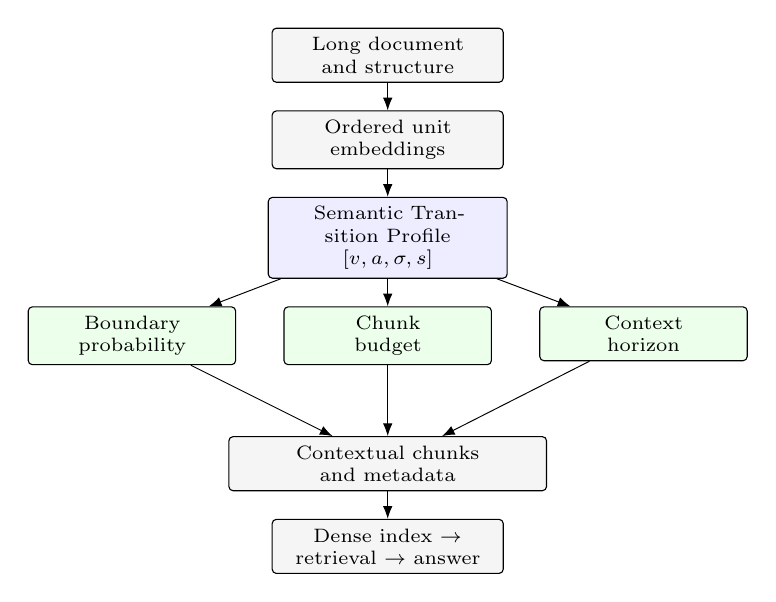
\begin{tikzpicture}[font=\scriptsize, node distance=3.5mm and 4mm, >=Latex,
 box/.style={draw, rounded corners=1.5pt, align=center, minimum height=6mm, text width=27mm, fill=gray!8},
 signal/.style={draw, rounded corners=1.5pt, align=center, minimum height=6mm, text width=28mm, fill=blue!7},
 decision/.style={draw, rounded corners=1.5pt, align=center, minimum height=6mm, text width=24mm, fill=green!8},
 line/.style={->, line width=.35pt}]
\node[box] (doc) {Long document\\and structure};
\node[box, below=of doc] (embed) {Ordered unit embeddings};
\node[signal, below=of embed] (stp) {Semantic Transition Profile\\$[v,a,\sigma,s]$};
\node[decision, below left=of stp] (bound) {Boundary\\probability};
\node[decision, below=of stp] (size) {Chunk\\budget};
\node[decision, below right=of stp] (ctx) {Context\\horizon};
\node[box, below=9mm of size, text width=38mm] (chunks) {Contextual chunks and metadata};
\node[box, below=of chunks] (index) {Dense index $\rightarrow$ retrieval $\rightarrow$ answer};
\draw[line] (doc)--(embed); \draw[line] (embed)--(stp);
\draw[line] (stp)--(bound); \draw[line] (stp)--(size); \draw[line] (stp)--(ctx);
\draw[line] (bound)--(chunks); \draw[line] (size)--(chunks); \draw[line] (ctx)--(chunks);
\draw[line] (chunks)--(index);
\end{tikzpicture}
\caption{STP is computed once per document unit and used to parameterise three preprocessing decisions.}
\label{fig:architecture}
\end{figure}

\subsection{Boundary and Granularity Policy}
The boundary probability after unit $u_i$ is calculated with a calibrated logistic function:
\begin{equation}
P(B_i=1)=\operatorname{sigmoid}(w_v\hat v_i+w_a\hat a_i+w_\sigma\hat\sigma_i+w_sS_i+b),
\end{equation}
where $S_i$ is a scalar structural-boundary score. A boundary is accepted only when its probability exceeds $\tau_B$ and the current chunk satisfies a minimum length $L_{\min}$. A maximum length $L_{\max}$ still forces a split, protecting indexability in very stable regions.

The local target budget uses positive acceleration because an increasing transition rate is more informative for a pending split than a decelerating one:
\begin{equation}
T_i=\alpha\hat v_i+\beta\max(\hat a_i,0)+\gamma\hat\sigma_i,
\end{equation}
\begin{equation}
L_i=\operatorname{clip}(L_{\max}-(L_{\max}-L_{\min})T_i,L_{\min},L_{\max}).
\end{equation}
Thus, stable regions receive larger budgets, while abrupt or volatile regions are represented more finely. Coefficients and thresholds should be selected on a held-out validation split, not tuned against the test set.

\subsection{Selective Context Propagation}
Chunk boundaries can remove material needed to interpret references such as ``this condition'' or an abbreviation defined earlier. Rather than appending a fixed number of predecessors, STP-RAG calculates a context horizon
\begin{equation}
H_i=\operatorname{clip}(H_{\min}+\lambda_1\hat\sigma_i+\lambda_2\max(\hat a_i,0)+\lambda_3R_i,H_{\min},H_{\max}),
\end{equation}
where $R_i$ is a reference/dependency signal. Candidate predecessors in the horizon are ranked using semantic similarity, dependency matching, and reference resolution. Only candidates exceeding a validation-selected threshold are attached as concise context. The indexed representation is $\tilde c_i=[c_i\Vert\mathrm{SelectedContext}_i]$, while the raw chunk and provenance metadata are retained separately for inspection.

\begin{algorithm}[t]
\caption{STP-Guided Contextual Chunking}
\label{alg:chunking}
\begin{algorithmic}[1]
\Require Document $D$, embedding model $E$, calibrated parameters $\Theta$
\Ensure Contextual chunks $C$
\State $U\gets\operatorname{ExtractStructureAwareUnits}(D)$
\State $E_U\gets\operatorname{Embed}(U,E)$; $S\gets\operatorname{StructureFeatures}(U)$
\State $P\gets\operatorname{ComputeSTP}(E_U,S)$
\State $C\gets\operatorname{Segment}(U,P,\Theta,L_{\min},L_{\max})$
\ForAll{$c_i\in C$}
  \State $H_i\gets\operatorname{ContextHorizon}(P_i,\Theta)$
  \State $X_i\gets\operatorname{SelectRelevantHistory}(C_{i-H_i:i-1},c_i)$
  \State $\tilde c_i\gets\operatorname{Augment}(c_i,X_i)$
\EndFor
\State \Return $\{\tilde c_i\}$ with raw-text provenance
\end{algorithmic}
\end{algorithm}

\section{Experimental Design}
\subsection{Research Questions and Baselines}
The evaluation should answer whether transition-aware chunking improves retrieval quality, question-answering quality, and efficiency without an impractical cost. Table~\ref{tab:ablations} defines the minimum comparison set. A fixed-size baseline must use the same embedding model, index, retrieval depth, and generator as STP-RAG so that chunk representation is isolated. A semantic-similarity baseline should use an explicitly stated threshold and the same chunk-length limits.

\begin{table}[t]
\caption{Minimum ablation plan. All systems should share the same corpus split, embedding model, index, retriever, and generation configuration.}
\label{tab:ablations}
\centering
\footnotesize
\begin{tabular}{p{20mm}ccc}
\toprule
System & $v$ & $a$ & $\sigma$ \\
\midrule
Fixed-size chunks & -- & -- & -- \\
Similarity-threshold chunks & distance only & -- & -- \\
Velocity-only & \checkmark & -- & -- \\
Velocity + acceleration & \checkmark & \checkmark & -- \\
Full STP & \checkmark & \checkmark & \checkmark \\
Full STP + selective context & \checkmark & \checkmark & \checkmark \\
\bottomrule
\end{tabular}
\end{table}

Suitable evaluation corpora include multi-hop QA benchmarks such as HotpotQA \parencite{yang2018hotpotqa} and domain-specific collections for which answer-bearing passages can be established. A legal-document extension may use CUAD for clause-oriented retrieval analysis \parencite{hendrycks2021cuad}; this extension should be reported separately because its task distribution differs from open-domain QA.

\subsection{Metrics and Protocol}
For retrieval, report Recall@1, Recall@5, Recall@10, and mean reciprocal rank (MRR), with an answer-bearing chunk or source passage defined before testing. For answer quality, report Exact Match and token-level F1 where benchmark annotations permit them. For efficiency, report average chunks per document, mean indexed tokens per chunk, index build time, and retrieval latency under identical hardware and batch settings.

Use a development split to choose $w$, $\tau_B$, chunk limits, and context thresholds. Freeze these values before testing. Run each configuration with at least three random seeds where the pipeline contains stochastic components, then report mean and standard deviation. Paired bootstrap confidence intervals or a paired permutation test can be used when query-level outputs are retained. Every run should record corpus version, embedding model version, random seed, and the exact prompt used for answer generation.

\section{Results Template and Reporting Guidance}
This paper intentionally does not invent numbers. Populate Table~\ref{tab:results} only after the evaluation protocol is executed. Empty cells are marked ``TBD'' rather than being presented as results. Once populated, the prose should distinguish observed findings from interpretation and should report negative or mixed outcomes as well as gains.

\begin{table*}[t]
\caption{Results template. Replace TBD only with measurements produced by the documented evaluation protocol. Report mean $\pm$ standard deviation when repeated runs are used.}
\label{tab:results}
\centering
\small
\begin{tabular}{lccccccc}
\toprule
Method & Recall@5 & MRR & EM & F1 & Chunks/doc. & Build time & Retrieval latency \\
\midrule
Fixed-size & TBD & TBD & TBD & TBD & TBD & TBD & TBD \\
Similarity-threshold & TBD & TBD & TBD & TBD & TBD & TBD & TBD \\
Velocity-only & TBD & TBD & TBD & TBD & TBD & TBD & TBD \\
Velocity + acceleration & TBD & TBD & TBD & TBD & TBD & TBD & TBD \\
Full STP & TBD & TBD & TBD & TBD & TBD & TBD & TBD \\
Full STP + selective context & TBD & TBD & TBD & TBD & TBD & TBD & TBD \\
\bottomrule
\end{tabular}
\end{table*}

The final discussion should answer three questions. First, does each additional signal improve at least one prespecified metric relative to velocity-only chunking? Second, is any quality change explained by a much larger index or unacceptable latency? Third, do gains vary by document structure, such as stable narrative text versus documents with dense definitions and exceptions? These questions prevent a single aggregate score from obscuring the mechanism under evaluation.

\section{Threats to Validity and Limitations}
STP is a hypothesis about useful control signals, not a guarantee that a kinematic analogy captures meaning. Embedding geometry depends on the chosen encoder; cosine distance can reflect style, boilerplate, or parser error rather than a meaningful topic shift. The meaning of $\Delta p_i$ also changes with unit granularity, so sentence-level and paragraph-level implementations should not be compared without care.

The method introduces parameters and implementation decisions that can overfit a single benchmark. Strict development/test separation and transparent ablations are therefore essential. Context propagation may improve dependency preservation while increasing index size or introducing irrelevant historical text. Finally, retrieval improvements do not automatically establish better answer faithfulness; answer evaluation should include evidence inspection or citation-grounded checks where feasible.

The present scope also excludes a claim of novelty for evidence-sufficiency routing or gap-targeted retrieval. Those components may be explored as downstream extensions, but the paper's primary claim is confined to STP-guided chunk construction and selective context selection.

\section{Conclusion}
This paper presents STP-RAG, a framework that represents local document dynamics through semantic velocity, acceleration, volatility, and structural cues. The profile is reused to guide chunk boundaries, chunk budgets, and selective context horizons. The contribution is deliberately framed as a measurable systems hypothesis rather than an absolute novelty claim: a shared transition profile may yield document representations that improve long-document RAG relative to fixed or single-signal chunking. The supplied ablation and reporting protocol provides a path to test that claim without fabricating results. Future work can assess whether the same profile is helpful at retrieval time, across domains, and with learned rather than calibrated decision functions.

\printbibliography
\end{document}
